\documentclass[12pt, a4paper, twoside]{article}
\usepackage[utf8]{inputenc}
\usepackage[cm]{fullpage}
\usepackage{fancyhdr}
\usepackage{textcomp}
\usepackage{graphicx}
\usepackage{amssymb}
\usepackage{listings}

\lstset{literate=
  {á}{{\'a}}1 {é}{{\'e}}1 {í}{{\'i}}1 {ó}{{\'o}}1 {ú}{{\'u}}1
  {Á}{{\'A}}1 {É}{{\'E}}1 {Í}{{\'I}}1 {Ó}{{\'O}}1 {Ú}{{\'U}}1
  {à}{{\`a}}1 {è}{{\`e}}1 {ì}{{\`i}}1 {ò}{{\`o}}1 {ù}{{\`u}}1
  {À}{{\`A}}1 {È}{{\'E}}1 {Ì}{{\`I}}1 {Ò}{{\`O}}1 {Ù}{{\`U}}1
  {ä}{{\"a}}1 {ë}{{\"e}}1 {ï}{{\"i}}1 {ö}{{\"o}}1 {ü}{{\"u}}1
  {Ä}{{\"A}}1 {Ë}{{\"E}}1 {Ï}{{\"I}}1 {Ö}{{\"O}}1 {Ü}{{\"U}}1
  {â}{{\^a}}1 {ê}{{\^e}}1 {î}{{\^i}}1 {ô}{{\^o}}1 {û}{{\^u}}1
  {Â}{{\^A}}1 {Ê}{{\^E}}1 {Î}{{\^I}}1 {Ô}{{\^O}}1 {Û}{{\^U}}1
  {œ}{{\oe}}1 {Œ}{{\OE}}1 {æ}{{\ae}}1 {Æ}{{\AE}}1 {ß}{{\ss}}1
  {ű}{{\H{u}}}1 {Ű}{{\H{U}}}1 {ő}{{\H{o}}}1 {Ő}{{\H{O}}}1
  {ç}{{\c c}}1 {Ç}{{\c C}}1 {ø}{{\o}}1 {å}{{\r a}}1 {Å}{{\r A}}1
  {€}{{\euro}}1 {£}{{\pounds}}1 {«}{{\guillemotleft}}1
  {»}{{\guillemotright}}1 {ñ}{{\~n}}1 {Ñ}{{\~N}}1}

\begin{document}

\title{Lista de exercícios sobre filtros de software}
\author{Cristiano Silva Júnior}
\date{23 de Junho de 2017}
\maketitle

\section{Filtro de média}

\subsection{Mostrar a derivação da forma recursiva.}

A partir da definição da média
$$\bar{x_k}=\frac{1}{k}\sum^{k}_{i=1}{x_i}$$
Podemos fazer a seguinte manipulação
$$\bar{x_k}=\frac{1}{k-1}\sum^{k-1}_{i=1}{x_i}+\frac{x_k}{k}$$
$$\bar{x_k}=(\frac{1}{k-1}\sum^{k-1}_{i=1}{x_i})\frac{k-1}{k}+\frac{x_k}{k}$$
Como
$$\bar{x_{k-1}}=\frac{1}{k-1}\sum^{k-1}_{i=1}{x_i}$$
Então
$$\bar{x_k}=\bar{x_{k-1}}\frac{k-1}{k}+\frac{x_k}{k}\square$$
% TODO Move QED square to the end of the line

\subsection{Implementação em MATLAB}

Para implementar o filtro dado em MATLAB, foi escrito o seguinte script:

\lstinputlisting[language=Matlab]{media1.m}

Para gerar os dados aleatórios de altitude, a seguinte função foi escrita:

\lstinputlisting[language=Matlab]{gerarEntrada.m}

Essas duas funções foram consolidadas em um script principal:

\begin{lstlisting}
% Gerando dados de entrada
[tempo altitude] = gerarEntrada();
limite = length(tempo);
mediaAtual = [ ];
for n = 1:limite
    mediaAtual(end+1) = media1(altitude(n));
end
% Plotando os gráficos
figure;
hold on;
plot(tempo, altitude, 'r');
plot(tempo, mediaAtual, 'b');
hold off;
\end{lstlisting}

A partir deste script, foi gerado o gráfico 1, onde a onda vermelha são os dados gerados aleatoriamente e em azul, temos a  média calculada.

\section{Filtro de média móvel}

\subsection{Derivação da fórmula recursiva}

Seguindo da definição de média móvel com janela de tamanho $n$,
$$\bar{x_k}=\frac{x_{k-n+1}+x_{k-n+2}+\ldots+x_{k-1}+x_{k}}{n}$$
É possível afirmar que
$$\bar{x_k}=\frac{x_{k-n}}{n} + \frac{x_{k-n+1}+x_{k-n+2}+\ldots+x_{k-1}+x_{k}}{n} -\frac{x_{k-n}}{n}$$
$$\bar{x_k}=\bar{x_{k-1}} + \frac{x_k}{n} - \frac{x_{k-n}}{n}\square$$


\subsection{Implementação em MATLAB}

Para implementar o filtro dado em MATLAB, foi escrito o seguinte script:

\lstinputlisting[language=Matlab]{media2.m}

Reaproveitando a entrada gerada na função $gerarEntrada()$, foi possível gerar o gráfico na figura 2.

\section{Filtro de média móvel ponderada}

\subsection{Derivação da fórmula recursiva}

Uma média móvel ponderada é definida por
$$\bar{x_k}=\alpha\bar{x_{k-1}}+(1-\alpha)x_k$$
onde $\alpha$ é um número real entre 0 e 1. Note que, se calcularmos $\bar{x_{k-1}}$, temos somente uma mudança de índices para realizar:
$$\bar{x_k-1}=\alpha\bar{x_{k-2}}+(1-\alpha)x_{k-1}$$
O mesmo acontece com $\bar{x_{k-2}}$:
$$\bar{x_k-2}=\alpha\bar{x_{k-3}}+(1-\alpha)x_{k-2}$$
Substituindo as médias anteriores na primeira equação:
$$\bar{x_{k-1}}=\alpha(\alpha\bar{x_{k-3}}+(1-\alpha)x_{k-2})+(1-\alpha)x_{k-1}$$
$$\bar{x_{k}}=\alpha(\alpha(\alpha\bar{x_{k-3}}+(1-\alpha)x_{k-2})+(1-\alpha)x_{k-1})+(1-\alpha)x_k$$
$$\bar{x_k}=\alpha^3\bar{x_{k-3}}+\alpha^2(1-\alpha)x_{k-2}+\alpha(1-\alpha)x_{k-1}+(1-\alpha)x_k\square$$

\subsection{Implementação em MATLAB}

Para implementar o filtro dado em MATLAB, foi escrito o seguinte script:

\lstinputlisting[language=Matlab]{media3.m}

Reaproveitando a entrada gerada na função $gerarEntrada()$, foi possível gerar o gráfico na figura 3.

\subsection{Discussão}

Nota-se que o filtro de média regular manteve sua média sempre no valor verdadeiro, haja visto que o ruído foi simulado para que ele obedecesse um comportamento gaussiano ao redor da altitude de 11000 metros. Isso pode parecer que este é o comportamento ideal de um filtro, mas não suporta bem as características de um sistema real.

Os outros dois filtros (de média móvel e média ponderada) funcionaram melhor neste sentido. Embora ambos estejam dependentes da determinação de um parâmetro (o tamanho da janela no caso do móvel; e o parâmetro $\alpha$ no caso do ponderado), eles atuam como filtros passa-baixa, acompanhando bem as oscilações do modelo real.

\begin{figure}
  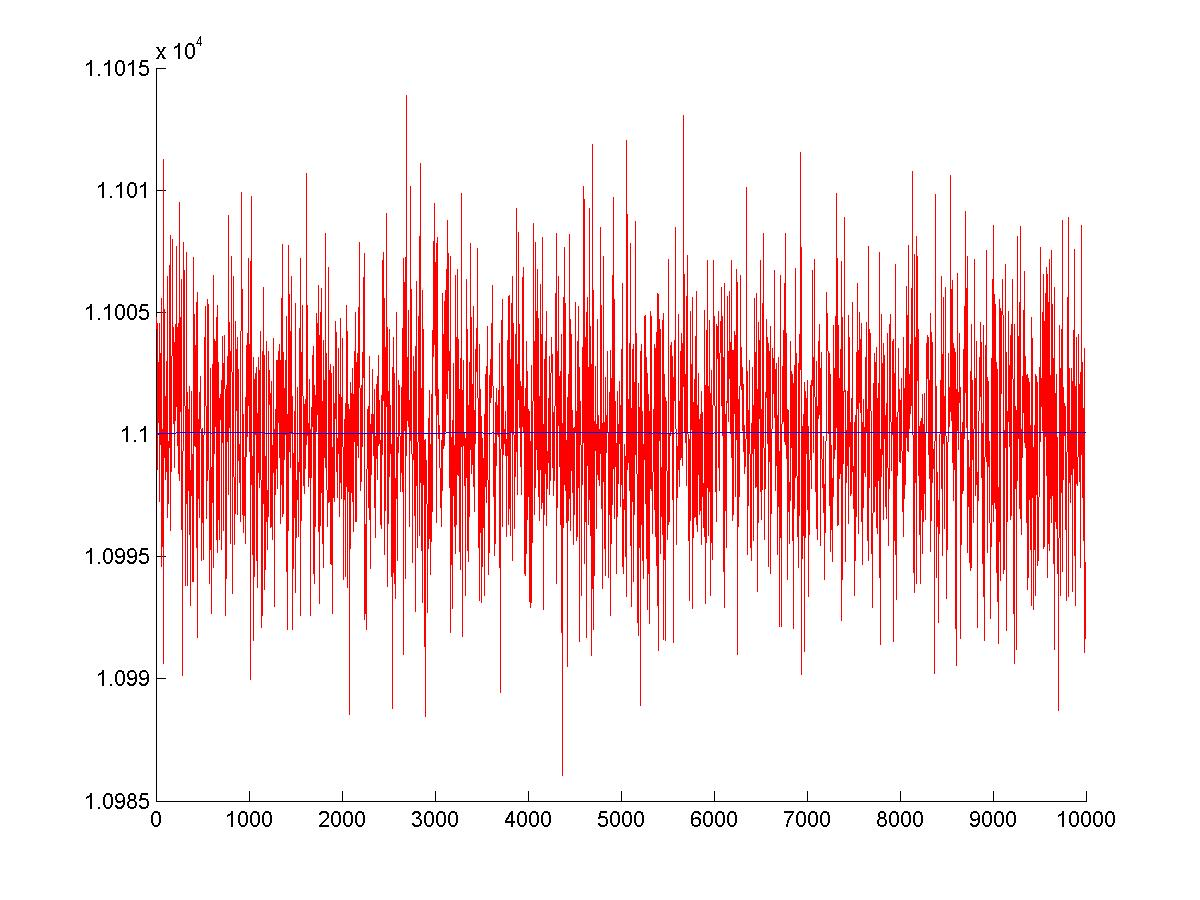
\includegraphics[width=0.9\textwidth]{mediaregular.jpg}
  \caption{Figura 1. Gráfico da média regular}
\end{figure}

\begin{figure}
  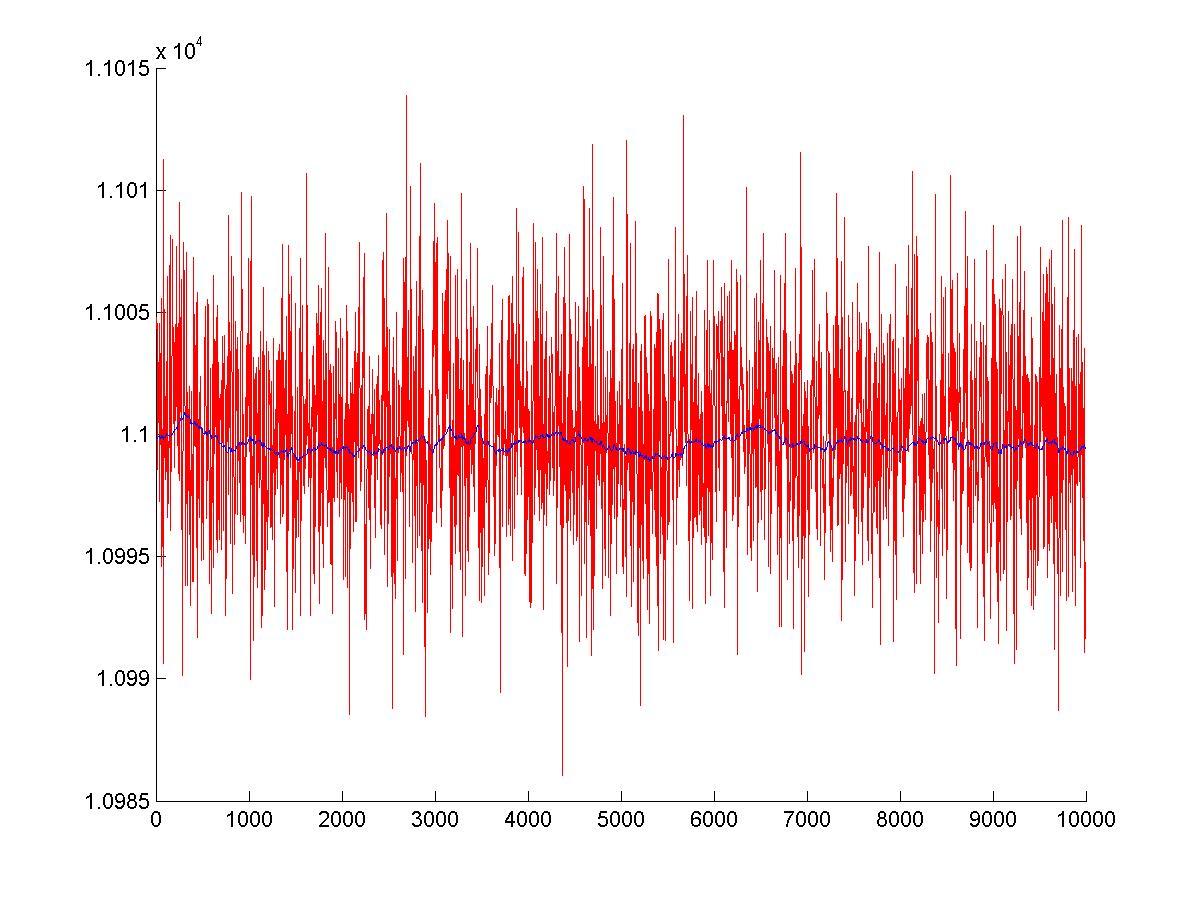
\includegraphics[width=0.9\textwidth]{mediamovel.jpg}
  \caption{Figura 2. Gráfico da média móvel}
\end{figure}

\begin{figure}
  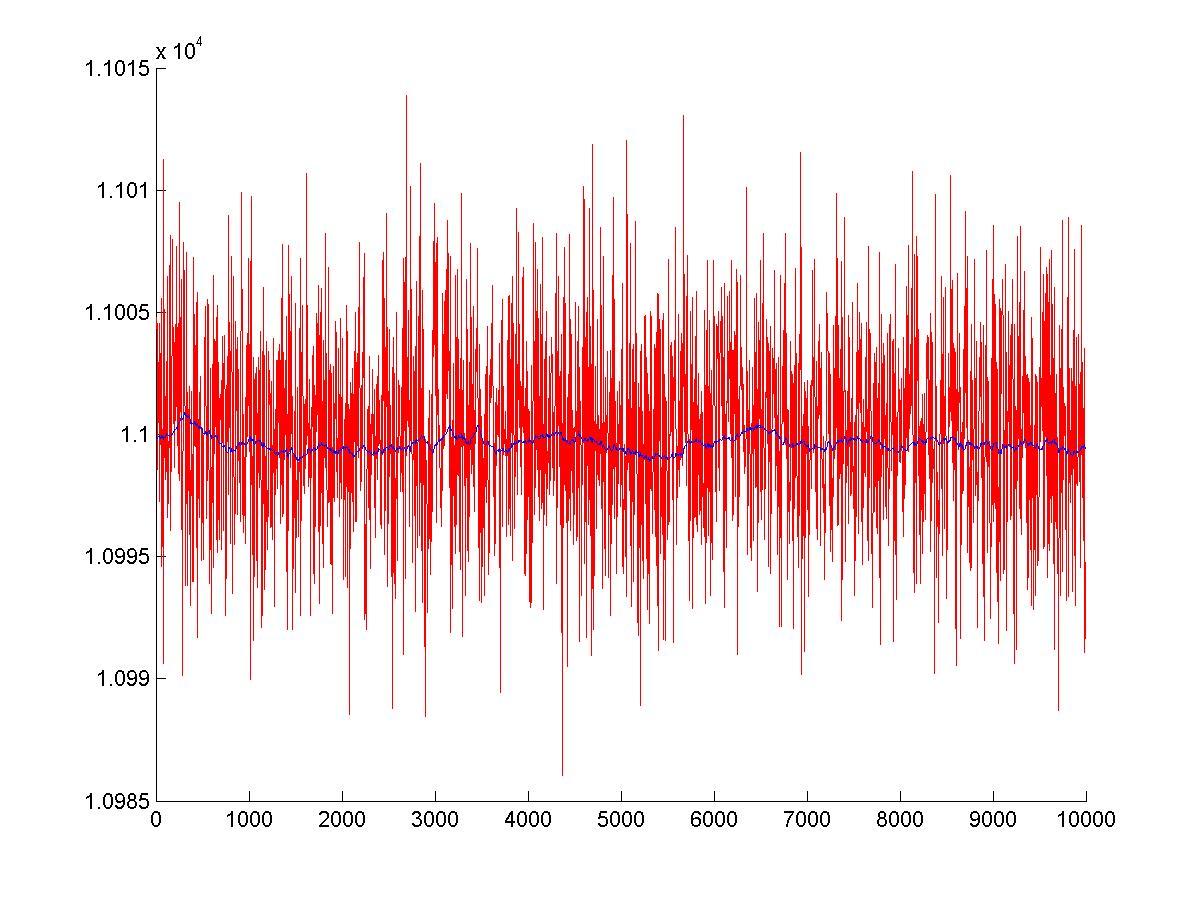
\includegraphics[width=0.9\textwidth]{mediamovel.jpg}
  \caption{Figura 3. Gráfico da média ponderada}
\end{figure}

\end{document}
